% !TeX root = Report.tex
\section{Implemented Algorithms}

\dirtree{%
.1 Common/.
.2 containers/.
.3 linked-list.[h/c].
.3 array-list.[h/c].
.3 unique-array.[h/c].
.3 map.[h/c].
.2 net/.
.3 eventupdate.[h/c].
.3 multipacket.[h/c].
.3 nhopflood.[h/c].
.3 nhopreq.[h/c].
.3 rimeaddr-helpers.[h/c].
.3 tree-aggregator.[h/c].
.2 debug-helper.[h/c].
.2 led-helper.[h/c].
.2 random-range.[h/c].
.2 sensor-converter.[h/c].
}

\subsection{Container Library}

Contiki comes with a list container \footnote{Header: \url{https://github.com/contiki-os/contiki/blob/master/core/lib/list.h} Source: \url{https://github.com/contiki-os/contiki/blob/master/core/lib/list.c}}, however, when we were developing with their linked list we found that it was awkward to use in some situations (for instance creating an array of lists) so we decided that we needed to find a better list library. Our problem was that other container libraries were unlikely to be optimised to the low memory requirements or support the special compile chain used by Contiki. So rather than waste time searching and integrating an external library we decided to write our own set of containers. By doing the main benefit we gained was that we knew how the containers worked so had a better understanding how to use them.

Another reason to develop our own containers was that we desired an list where the data was stored in an array, this was for because it provides lower memory overhead and the types of operations we would be performing (append and empty) meant that an array backed list would be better. The lower memory overhead comes from the fact that an array-based list doesn't need to store a pointer to the next element as it is implicit (due to the contiguous memory) that a pointer to the current element's pointer plus one is the next element. This means that in a list of $N$ items our singly linked list implementation will require $(\text{sizeof}(T) + \text{sizeof}(void *) \times 2) \times N$ bytes of memory, whereas our array list implementation will require $(\text{sizeof}(T) + \text{sizeof}(void *)) \times N$ bytes of memory.

Our linked list implementation uses more memory compared to Contiki's implementation because their list is \emph{intrusive}\footnote{Boost Containers: \url{http://www.boost.org/doc/libs/1\_53\_0/doc/html/intrusive/presenting\_containers.html}}. What is meant by this is that the pointer to the next item in the list is contained in the structure stored in the list \cite{?}. Meaning their list uses the same amount of memory as our array list. However, because the list is intrusive it makes it more difficult to use as the implementation detail leaks into the structure using the library, this was why developing our own non-intrusive list made it easier to develop code.

We also developed containers that helped abstract certain concepts (such as list uniqueness or accessing elements by key) to decrease code duplication and allow us to express the code in a higher-level way making implementation easier. One thing to note is that for the containers we did not focus on implementing some of their functions to the standard complexity. For example our map implementation has requires O(N) for both insert and fetching, where these may be implemented as O(1) on average (hash tables) or O(log N) (trees), however due to the requirements of low memory we decided to keep using the array as the backing store for the data with the aim to keep memory for at the expense of non-optimal container management functions. The increased time complexity should make little difference as the containers tend to have few elements in them (i.e. hundreds rather than millions, where complexity would start to be important \cite{?}).

Finally, all of these custom containers are tested by a test suite that checks for functional correctness. Also the test suite was run using \verb|valgrind|\footnote{\url{http://valgrind.org/info/tools.html}} to check for memory leaks and corruption.

\subsection{Network Library}

In order to facilitate the development of our predicate checking algorithms, numerous separate libraries that encapsulated specific functionality needed to be implemented. The reason that these algorithms and protocols were implemented as libraries was so that our code remained well encapsulated, leading to easier testing and development.

\subsubsection{Multi-Packet Unicast}

In Contiki sending a single packet has its limits, there is only so much data you can get in a single packet. There are two C macros that are relevant to this \verb|PACKETBUF_HDR_SIZE| which is set to 48 bytes and \verb|PACKETBUF_SIZE| which is set to 128 bytes\footnote{packetbuf.h \url{http://contiki.sourceforge.net/docs/2.6/a00302.html}}. This means that in general we will only be able to send a packet containing 128 bytes of information. But if a protocol called for sending a data structure that spans more than 128 bytes bytes, then a way to send multiple packets and a receiver that can put the packets back together in the correct way to deliver the data is required.

Contiki's data transfer primitives for their Rime protocols are fairly hidden because of their focus on uIPv6. We found \verb|ruldolph0| first \footnote{ruldolph0 \url{http://contiki.sourceforge.net/docs/2.6/a01735.html}} and then \verb|rucb| (Reliable Unicast Bulk Transfer) much later \footnote{rucb \url{http://contiki.sourceforge.net/docs/2.6/a00365.html}}. However, both of them have problems, both APIs are very convoluted and seem more geared towards sending very large files across the network. This is very different to our aim, which is to send relatively small packets of data to a specific neighbour. So we wrote our own API that would split data of any given size and reassemble it once received, our API was not focused on processing data chunks like \verb|ruldolph0| or \verb|rucb|, but simply operated on a block of memory given to it. This is a case where a simpler API made development much easier for us. Admittedly because our implementation uses dynamic memory allocation it could potentially perform worse, but because the energy of sending and receiving messages dwarfs the energy usage of the CPU, we feel that easier development tradeoff made it worth it. Also, now that code has been written to use this API, the \verb|multipacket| library itself could always be rewritten to use \verb|rucb| as a base to run more efficiently.

\subsubsection{N-Hop Request} 

We developed the N-Hop Request communication layer very early in the project. Our application needed a way to ask neighbouring nodes for information, and these messages sometimes needed to travel multiple hops in the network to do so. Initially we consulted the Contiki libraries to see if any of the existing network primitives could be used for this purpose.

We first considered \verb|Mesh| which sends a packet to any node on the network, this seemed like it would be a prefect fit for sending data back to the originator node. However, issues arose when we discovered that it could only send one unique packet across the network at a time. This was due to the way that \verb|Mesh| was implemented, it only maintains a record of the most recently received packet on the network. This assumption is fine if you assume that you only have 1 sender like a base station but when you have multiple senders sending different packets it fails. This could only have been scaled by having a \verb|Mesh| connection per node, which is not scalable at all. Next we considered \verb|Trickle| \footnote{trickle.h \url{http://contiki.sourceforge.net/docs/2.6/a00381.html}}. Unfortunately, like \verb|Mesh|, \verb|Trickle| had similar shortcomings which made unsuitable for our task.

Having explored several options from the Contiki source library we realised that N-Hop Request had a very specific set of requirements. We found that no one library offered all the functionality we needed; Therefore, We opted for developing our own communication layer and API to handle the routing of these messages. The layer would need to flood the network, a fixed number of hops from the source, whilst allowing multiple nodes to use the same layer, with different messages. For this we built upon Contiki Rime communication libraries.

The libraries that we used were \verb|stbroadcast| (Stubborn Broadcast) and \verb|runicast| (Reliable Unicast). Stubborn Broadcast is used to send the request data messages n-hops into the network. Every node that receives the request checks the time-to-live (ttl) of the message; if it is greater than 1 then, it decrements the ttl and forwards the packet on to it's neighbours. Stubborn Broadcast was used as it broadcasts a message at a given rate, allowing this to send a few copies of the message at random intervals increases the chance that the message will be received by the neighbours. To keep energy costs down the number of message repeats is kept low.

When a node receives a request message it keeps a record of from what node it came from and which node is requesting the information, this is so that when replies are being sent they can simply follow this path instead of being broadcasted. After this information has been stored the node then waits a fixed amount of time before sending a reply. This is done so that request messages have time to propagate away to avoid collisions. Once the timer times-out Reliable Unicast is then used to send the reply to the neighbour recorded as being on the path to the node that requested this information. Reliable Unicast is used in attempt to provide reliable transmission and reduce energy usage, as in the best case it will simply involve the overhead of a single ack message.

If a node receives the reply packet and isn't the intended target (the originator) they forward the packet onto the node that they received their request message from, eventually the packet will arrive back at the originator who can then deliver the message. In order to minimise message sends, each node maintains the most efficient node to get back to the originator. This is based on the number of hops it takes for a request message to reach the node, a message from a node with 3 hops left is a more efficient route than a message from a node with only 2 hops left. Finally, once a pre-determined wait period has expired the gathered data is passed to the predicate evaluator and any further data received is not delivered.

\begin{figure}[H]
\centering
\subfigure[Flooding request message two hops]{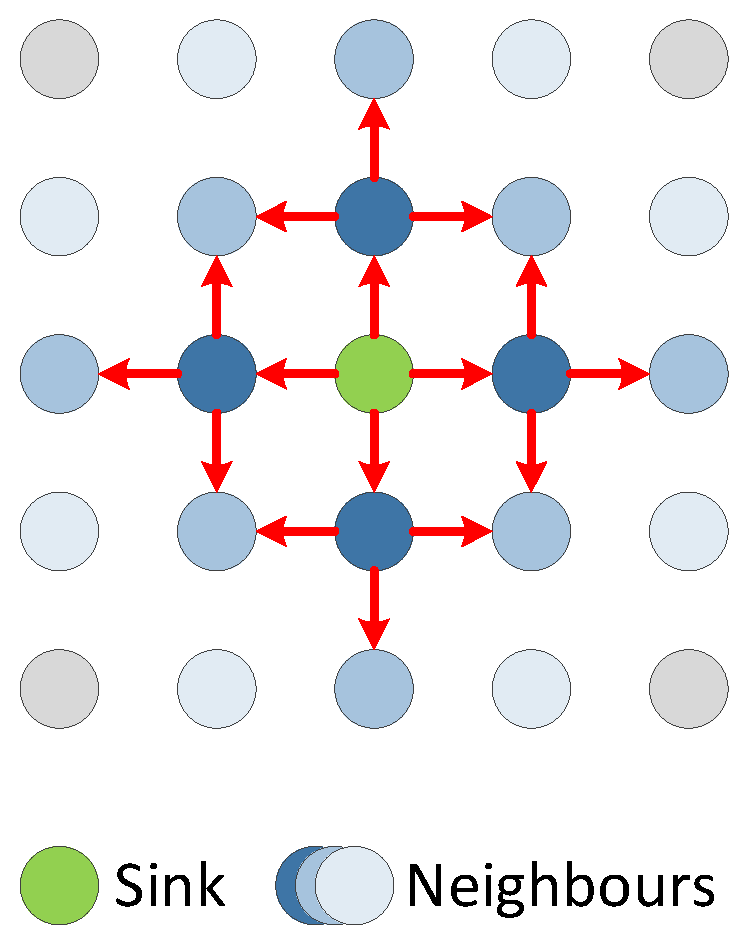
\includegraphics[scale=0.5]{Diagrams/2-hop-flooding.eps}}\hspace{5em}
\subfigure[Single path of a request and replies]{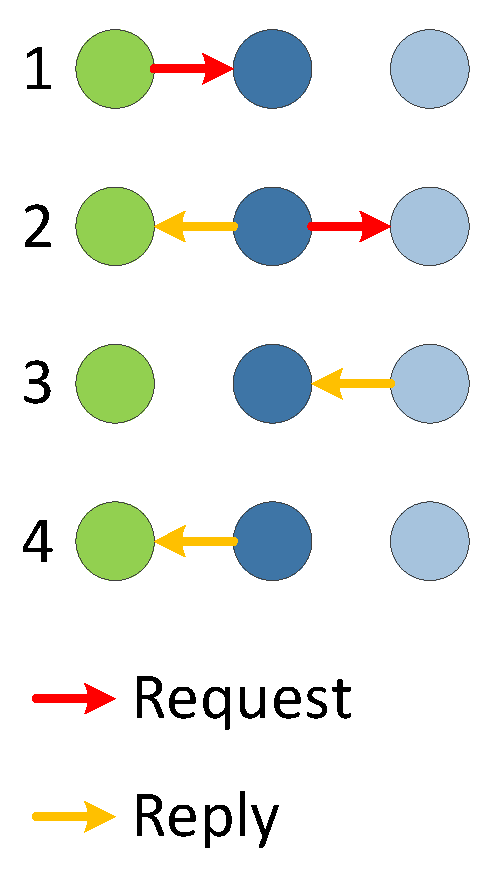
\includegraphics[scale=0.5]{Diagrams/n-hop-flood-req-reply.eps}}
\caption{Example of N-Hop Flood when N=2}
\end{figure}

%TODO: Note about performance maybe?

\begin{figure}[H]
  \centering
  \begin{boxedminipage}{\linewidth}
    % 
    \null Process $j$ - \res{n-hop-req}\\
    %
    %
    \null \textbf{variables}\\
    %
    \null\qq \%The key is the node this entry is about.\\
    \null\qq \%The entry contains how many hops away the node is,\\
    \null\qq \%what node a reply should be forwarded to and the message id the entry is relevant to.\\
    \null\qq \var{records}: map of address to (\var{hops}: int, \var{forwardTo}: address, \var{id}: int) init $\emptyset$;\\~\\
    %
    \null\qq \var{messageId}: int init 1;\\~\\
    %
    \null\qq \var{sendData}: timer init $\bot$;\\~\\
    %
    %
    \null \textbf{constants}\\
    %
    \null\qq \% Send Data Period, the time between receiving a request for data, and sending it\\
    \null\qq \var{$P_{sendData}$}: time;\\~\\
    %
    %
    \null \textbf{actions}\\
    %
    %
    \null\qq \% Sending Data Request Message\\
    \null\qq \emph{nhopreq.send}::~\res{function}$\langle \var{hops}\rangle\rightarrow$\\
    \null\qq\qq \res{bcast}$\langle \var{j}, \var{j}, \var{messageId}, \var{hops}, 0\rangle$;\\
    \null\qq\qq $\var{messageId} \assign \var{messageId} + 1$;\\~\\
    %
    %
    \null\qq \% Receiving Data Request Message\\
    \null\qq \emph{receiveRequest}::~\res{recv}$\langle originator, sender, id, ttl, hops\rangle \rightarrow$\\
    \null\qq\qq \res{if} ($\var{originator} \not= \var{j}$) \res{then}\\
    \null\qq\qq\qq $\var{respond} \assign False$;\\
    \null\qq\qq\qq \res{if} ($\var{originator} \in \res{keys}(\var{records})$) \res{then}\\
    \null\qq\qq\qq\qq $(\var{recHops}, \var{recForwardTo}, \var{recId}) \assign \var{records}[\var{originator}]$;\\
    \null\qq\qq\qq\qq \res{if} ($\var{hops} < \var{recHops}$) \res{then}\\
    \null\qq\qq\qq\qq\qq $\var{records}[\var{originator}] \assign (\var{hops}, \var{sender}, \var{recId})$;\\
    \null\qq\qq\qq\qq \res{fi}; \\
    \null\qq\qq\qq\qq $(\var{recHops}, \var{recForwardTo}, \var{recId}) \assign \var{records}[\var{originator}]$;\\
    \null\qq\qq\qq\qq \res{if} ($\var{id} > \var{recId}$) \res{then}\\
    \null\qq\qq\qq\qq\qq $\var{records}[\var{originator}] \assign (\var{recHops}, \var{recForwardTo}, \var{id})$;\\
    \null\qq\qq\qq\qq\qq $\var{respond} \assign True$;\\
    \null\qq\qq\qq\qq \res{fi}; \\
    \null\qq\qq\qq \res{else}\\
    \null\qq\qq\qq\qq $\var{records}[\var{originator}] \assign (\var{hops}, \var{sender}, \var{id})$;\\
    \null\qq\qq\qq\qq $\var{respond} \assign True$;\\
    \null\qq\qq\qq \res{fi;}\\
    \null\qq\qq\qq \res{if} ($respond$)\\
    \null\qq\qq\qq\qq $(\var{recHops}, \var{recForwardTo}, \var{recId}) \assign \var{records}[\var{originator}]$;\\
    \null\qq\qq\qq\qq \res{unicast.send}$\langle originator, j, 0, \res{NodeData}() \rangle$ \res{to} \var{recForwardTo};\\
    \null\qq\qq\qq\qq \res{bcast}$\langle \var{originator}, \var{j}, \var{id}, \var{hops} - 1, \var{hops} + 1\rangle$;\\
    \null\qq\qq\qq \res{fi;}\\
    \null\qq\qq \res{fi;}\\~\\
    %
    %
    \null\qq \% Received Data Forward Message\\
    \null\qq \emph{forwardData}::~\res{unicast.recv}$\langle target, sender, hops, data\rangle \rightarrow$\\
    \null\qq\qq $(\var{recHops}, \var{recForwardTo}, \var{recId}) \assign \var{records}[\var{target}]$;\\
    \null\qq\qq \res{if} ($\var{j} = \var{target}$) \res{then}\\
    \null\qq\qq\qq \res{nhopreq.deliver}(\var{sender}, \var{hops}, \var{data});\\
    \null\qq\qq \res{else}\\
    \null\qq\qq\qq \res{unicast.send}$\langle target, sender, hops + 1, data \rangle$ \res{to} \var{recForwardTo};\\
    \null\qq\qq \res{fi;}\\
    %
    %
  \end{boxedminipage}
  \caption{N-Hop Request Algorithm}
  \label{fig:n-hop-req-algorithm}
\end{figure}

\subsubsection{N-Hop Flood}

The previously mentioned algorithm was developed so that nodes could ask for information from its N-hop neighbourhood when it is needed. This was used for when predicates were asking for data periodically, however, if nodes are sending data when said data changes then N-hop request is not as applicable. Therefore, we developed N-hop flood, which floods information the required N hops.

The N-Hop Flood protocol keeps a queue of the messages that it needs to send. Every $P_{send}$ period it will broadcast what is on the top of the queue and increment the number of times that message had been sent. Once a message reaches the maximum number of retransmits it is removed from the queue. New messages are appended to the end of the queue so they are sent after messages added to the queue earlier.

When a node receives a flooded message it checks to see what the time-to-live (TTL) of the message is. If it is not 0 then that  the message is added to the queue to continue being forwarded. The node will also check the id included within the message. If the node had not received a message with that id from the sender before or it had received a message from that sender but from a route that was longer the message is delivered to the user of the library.

\begin{figure}[H]
  \centering
  \begin{boxedminipage}{\linewidth}
    % 
    \null Process $j$ - \res{n-hop-flood}\\
    %
    \null \textbf{parameters}\\
    %
    \null\qq \% The send period for this predicate\\
    \null\qq \var{$P_{send}$}: time;\\~\\
    %
    \null\qq \% The max number of times to re-transmit\\
    \null\qq \var{maxretx}: int;\\~\\
    %
    %
    \null \textbf{variables}\\
    %
    \null\qq \var{id}: int init 0;\\~\\
    %
    \null\qq \var{sendData}: timer init \var{$P_{send}$};\\~\\
    %
    \null\qq \% The queue of packets that need to be broadcast\\
    \null\qq \% Tuple contains: (id, sender, ttl, hops, retx, data)\\
    \null\qq \var{packetQueue}: queue of (int, address, int, int, int, struct) init $\emptyset$;\\~\\
    %
    \null\qq \% The map of all messages received from the nodes N-Hop neighbours\\
    \null\qq \% The entry contains a tuple of (packet id, hops)\\
    \null\qq \var{seen}: map of address to (int, int) init $\emptyset$;\\
  \end{boxedminipage}
  \caption{N-Hop Flood Algorithm}
  \label{fig:n-hop-flood-algorithm}
\end{figure}
\begin{figure}[H]
  \centering
  \begin{boxedminipage}{\linewidth}
    %
    %
    \null \textbf{actions}\\
    %
    %
    \null\qq \% Sending Message\\
    \null\qq \emph{nhopflood.send}::~\res{function}$\langle \var{data}, \var{hops}\rangle\rightarrow$\\
    \null\qq\qq \res{if} ($hops \not= 0$) \res{then}\\
    \null\qq\qq\qq \res{append}(\var{packetQueue}, (\var{id}, j, \var{hops}, 0, 0, \var{data})); \\
    \null\qq\qq\qq $\var{id} \assign \var{id} + 1$; \\
    \null\qq\qq \res{fi;}\\~\\
    %
    %
    \null\qq \emph{check}::~\res{timeout}(\var{sendData}) $\rightarrow$\\
    \null\qq\qq $\var{top} \assign \res{peek}(\var{packetQueue})$;\\
    \null\qq\qq \res{if} ($\var{top} \not= \bot$) \res{then}\\
    \null\qq\qq\qq $(id, sender, ttl, hops, retx, data) \assign \var{top}$;\\
    \null\qq\qq\qq \res{if} ($\var{top} \not= \bot$) \res{then}\\
    \null\qq\qq\qq\qq \res{bcast}$\langle sender, hops + 1, ttl - 1, id, data\rangle$;\\
    \null\qq\qq\qq\qq $\var{retx} \assign \var{retx} + 1$;\\
    \null\qq\qq\qq \res{fi};\\
    \null\qq\qq\qq \res{pop}(\var{packetQueue});\\
    \null\qq\qq\qq \res{if} ($\var{retx} < \var{maxretx} \land \var{ttl} > 0$) \res{then}\\
    \null\qq\qq\qq\qq \res{prepend}(\var{packetQueue}, $(id, sender, ttl, hops, retx, data)$);\\
    \null\qq\qq\qq \res{fi}; \\
    \null\qq\qq \res{fi;}\\
    \null\qq\qq \res{set}(\var{sendData}, \var{$P_{send}$}); \\~\\
    %
    %
    \null\qq \% Receive Message\\
    \null\qq \emph{recvData}::~\res{recv}$\langle originator, hops, ttl, id, data\rangle \rightarrow$\\
    \null\qq\qq $\var{seenBefore} \assign True$;\\
    \null\qq\qq \res{if} ($\var{originator} \not\in \res{keys}(\var{seen}) $) \res{then}\\
    \null\qq\qq\qq $\res{seen}[\var{originator}] \assign (id, hops)$;\\
    \null\qq\qq\qq $\var{seenBefore} \assign False$;\\
    \null\qq\qq \res{else} \\
    \null\qq\qq\qq $(seenId, seenHops) \assign \res{seen}[\var{originator}]$;\\
    \null\qq\qq\qq \res{if} ($\var{seenId} < \var{id}$) \res{then}\\
    \null\qq\qq\qq\qq $\res{seen}[\var{originator}] \assign (id, hops)$;\\
    \null\qq\qq\qq\qq $\var{seenBefore} \assign False$;\\
    \null\qq\qq\qq \res{else if} ($\var{seenId} = \var{id} \land \var{seenHops} > \var{hops}$) \res{then}\\
    \null\qq\qq\qq\qq \res{nhopflood.deliver}(\var{originator}, \var{hops}, \var{seenHops}, \var{data});\\
    \null\qq\qq\qq\qq $\res{seen}[\var{originator}] \assign (seenId, hops)$;\\
    \null\qq\qq\qq \res{fi};\\
    \null\qq\qq \res{fi;}\\
    \null\qq\qq \res{if} ($\lnot\var{seenBefore}$) \res{then}\\
    \null\qq\qq\qq \res{nhopflood.deliver}($\var{originator}, \var{hops}, 0, \var{data}$);\\
    \null\qq\qq\qq \res{if} ($\var{ttl} > 0$) \res{then}\\
    \null\qq\qq\qq\qq \res{append}(\var{packetQueue}, (\var{id}, \var{originator}, \var{ttl}, \var{hops}, 0, \var{data})); \\
    \null\qq\qq\qq \res{fi};\\
    \null\qq\qq \res{fi;}\\
    %
    %
  \end{boxedminipage}
  \caption{N-Hop Flood Algorithm}
  \label{fig:n-hop-flood-algorithm}
\end{figure}

\subsubsection{Event Update}

The event update library was developed for use with predicates being evaluated locally in-network where information needed to be disseminated a given number of hops once the mote's data changed. This library periodically generates the current state of the mote and then checks it against the previously sent state. If there is no previously sent state or the state has changed as specified by a $\var{differs}$ function, then the recently generated state is flooded the required distance. For our usage this distance will be the maximum number of hops that a predicate needs information from.

\begin{figure}[H]
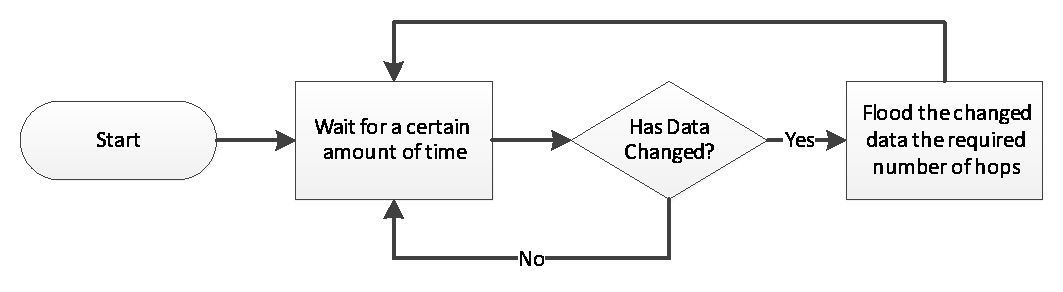
\includegraphics[width=\linewidth]{Diagrams/event-update-flowchart.eps}
\caption{Process of event update sending changed data}
\end{figure}

\begin{figure}[H]
  \centering
  \begin{boxedminipage}{\linewidth}
    % 
    \null Process $j$ - \res{event-update}\\
    %
    \null \textbf{variables}\\
    %
    \null\qq \var{period}: timer init $P_{generate}$;\\~\\
    %
    \null\qq \% The previous node data sent to the network\\
    \null\qq \var{previous}: struct init $\bot$;\\~\\
    %
    \null \textbf{constants}\\
    %
    \null\qq \% Generate Period, how often we should check for a change in the data\\
    \null\qq \var{$P_{generate}$}: time;\\~\\
    %
    \null\qq \% Checks if the data differs\\
    \null\qq \var{differs}: function takes (struct, struct) returns boolean;\\~\\
    %
    \null\qq \% Gets the data of the current node\\
    \null\qq \var{data}: function takes () returns struct;\\~\\
    %
    \null\qq \% The probability of sending our data, even if no change occurred\\
    \null\qq \var{chance}: real;\\~\\
    %
    \null \textbf{parameters}\\
    %
    \null\qq \% The distance we need to send information\\
    \null\qq \var{distance}: int;\\~\\
    %
    \null \textbf{actions}\\
    %
    %
    \null\qq \% Check for changes\\
    \null\qq \emph{check}::~\res{timeout}(\var{period}) $\rightarrow$\\
    \null\qq\qq $\var{force} \assign \res{RandReal}(0, 1) \leq \var{chance}$;\\
    \null\qq\qq $\var{changed} \assign \var{previous} = \bot \lor \var{differs}(\var{data}(), \var{previous})$;\\
    \null\qq\qq \res{if} ($\var{force} \lor \var{changed}$) \res{then}\\
    \null\qq\qq\qq $\var{previous} \assign \var{data}()$;\\
    \null\qq\qq\qq \res{nhopflood.send}$\langle j, \var{previous}, \var{distance}\rangle$;\\
    \null\qq\qq \res{fi}; \\
    \null\qq\qq \res{set}($\mathit{period}$, $P_{generate}$); \\~\\
    %
    %
    \null\qq \% Receiving Change message\\
    \null\qq \emph{receive}::~\res{nhopflood.recv}$\langle source, data, hops\rangle \rightarrow$\\
    \null\qq\qq \% Prevent delivery if being told that the current node's data has changed\\
    \null\qq\qq \res{if} ($j \not= source$) \res{then} \\
    \null\qq\qq\qq \% Inform library caller of data change\\
    \null\qq\qq\qq \res{event-update.callback}(\var{data}, \var{hops}); \\
    \null\qq\qq \res{fi}; \\
    %
    %
  \end{boxedminipage}
  \caption{Event Update Broadcast Algorithm}
\end{figure}


\subsubsection{Tree Aggregation}

As has been previously mentioned Tree Aggregation is a very useful technique employed in wireless sensor networks to aggregate a set of data to a single node in the network. It is very useful because of its ability to convey the same amount of data in potentially fewer messages. The algorithm works by first creating a tree structure such that nodes know of a parent node that they should unicast their messages to. Once this tree is set up the nodes (typically leaf nodes) unicast data to their parents, this can either happen when an event occurs or it can happen periodically. When a parent node receives a message it waits for a certain amount of time for more messages to arrive, every message it receives is stored and aggregated. After the time period is up the aggregated data is forwarded to its parent node. Once the data reaches the destination it is delivered to the user of the library.


The user of this library needs to implement four important functions:
\begin{enumerate}
\item[$\otimes_{agg}$] This function aggregates stored data with data message that has been received
\item[$\otimes_{own}$] This function aggregates the node's own data into the stored data
\item[$\otimes_{read}$] This function does the initial reading of data from a message and creates the local stored data
\item[$\otimes_{write}$] This function writes the local stored data back to a packet
\end{enumerate}


\begin{figure}[H]
  \centering
  \begin{boxedminipage}{\linewidth}
    % 
    \null Process $j$ - \res{tree-aggregation}\\
    %
    \null \textbf{variables}\\
    %
    \null\qq \var{parentdetect}: timer init $\bot$;\\~\\
    %
    \null\qq \var{seensetup}, \var{collecting}, \var{leaf}: bool init $False$, $False$, $True$;\\~\\
    %
    \null\qq \var{besthop}: int init $INTMAX$;\\~\\
    %
    \null\qq \var{bestparent}: address init $\bot$;\\~\\~\\
    %
    \null\qq \var{aggregation}: timer init $\bot$;\\~\\
    %
    \null\qq \var{collecting}: bool init $False$;\\~\\
    %
    \null\qq \var{stored}: struct init $\bot$;\\~\\
    %
    \null \textbf{constants}\\
    %
    \null\qq \% How long to wait for messages to aggregate before forwarding what the node has\\
    \null\qq \var{$P_{aggregation}$}: time;\\~\\
    %
    \null\qq \% How long to wait for parents to be detected\\
    \null\qq \var{$P_{parentdetect}$}: time;\\~\\
    %
    \null \textbf{parameters}\\
    %
    \null\qq \% The address of the node data should be aggregated to\\
    \null\qq \var{sink}: address;\\
    %
  \end{boxedminipage}
  \caption{Tree Aggregation Algorithm - variables}
\end{figure}

\begin{figure}[H]
  \centering
  \begin{boxedminipage}{\linewidth}
    \null \textbf{actions}\\
    %
    %
    \null\qq \% Set up tree: initialise\\
    \null\qq \emph{starup}::~\res{init} $\rightarrow$\\
    \null\qq\qq \res{bcast}$\langle j, \bot, 1\rangle$;\\~\\
    %
    %
    \null\qq \% Set up tree: receive message\\
    \null\qq \emph{receive}::~\res{recv}$\langle source, parent, hops\rangle \rightarrow$\\
    \null\qq\qq \res{if} ($j \not= sink$) \res{then} \\
    \null\qq\qq\qq \res{if} ($\lnot\var{seensetup}$) \res{then} \\
    \null\qq\qq\qq\qq $\var{seensetup} \assign True$; \\
    \null\qq\qq\qq\qq \res{set}($\mathit{parentdetect}$, $P_{parentdetect}$); \\
    \null\qq\qq\qq \res{fi}; \\
    \null\qq\qq\qq \res{if} ($\var{hops} < \var{besthop}$) \res{then} \\
    \null\qq\qq\qq\qq $\var{bestparent}, \var{besthop} \assign \var{source}, \var{hops}$; \\
    \null\qq\qq\qq \res{fi}; \\
    \null\qq\qq\qq \res{if} ($\var{leaf} \land \var{j} = \var{parent}$) \res{then} \\
    \null\qq\qq\qq\qq $\var{leaf} \assign False$; \\
    \null\qq\qq\qq \res{fi}; \\
    \null\qq\qq \res{fi}; \\~\\
    %
    %
    \null\qq \% Set up tree: finish detecting parents\\
    \null\qq \emph{check}::~\res{timeout}(\var{parentdetect}) $\rightarrow$\\
    \null\qq\qq \res{if} ($\var{besthop} = INTMAX$) \res{then} \\
    \null\qq\qq\qq \res{bcast}$\langle j, \var{bestparent}, INTMAX\rangle$;\\
    \null\qq\qq \res{else} \\
    \null\qq\qq\qq \res{bcast}$\langle j, \var{bestparent}, \var{besthop} + 1\rangle$;\\
    \null\qq\qq \res{fi};
    %
    %
  \end{boxedminipage}
  \caption{Tree Aggregation Algorithm - Setting up tree}
\end{figure}


\begin{figure}[H]
  \centering
  \begin{boxedminipage}{\linewidth}
    \null \textbf{actions}\\
    %
    %
    \null\qq \% Send data function\\
    \null\qq \emph{treeagg.send}::~\res{function}$\langle data\rangle \rightarrow$\\
    \null\qq\qq \res{multipacket.send}$\langle j, data\rangle$ \res{to} \var{bestparent};\\~\\
    %
    %
    \null\qq \% Set up tree: receive message\\
    \null\qq \emph{receive}::~\res{multipacket.recv}$\langle source, data\rangle \rightarrow$\\
    \null\qq\qq \res{if} ($j = sink$) \res{then} \\
    \null\qq\qq\qq $\var{stored} \assign \otimes_{read}(data)$; \\
    \null\qq\qq\qq $\var{stored} \assign \otimes_{own}(\var{stored})$; \\
    \null\qq\qq\qq $\res{treeagg.deliver}(\otimes_{write}(\var{stored}))$; \\
    \null\qq\qq \res{else} \\
    \null\qq\qq\qq \res{if} ($\var{collecting}$) \res{then} \\
    \null\qq\qq\qq\qq $\var{stored} \assign \otimes_{agg}(\var{stored}, \var{data})$; \\
    \null\qq\qq\qq \res{else} \\
    \null\qq\qq\qq\qq $\var{stored} \assign \otimes_{read}(data)$; \\
    \null\qq\qq\qq\qq $\var{collecting} \assign True$; \\
    \null\qq\qq\qq\qq \res{set}($\var{aggregation}$, $P_{aggregation}$); \\
    \null\qq\qq\qq \res{fi}; \\
    \null\qq\qq \res{fi}; \\~\\
    %
    %
    \null\qq \% Set up tree: finish detecting parents\\
    \null\qq \emph{finishagg}::~\res{timeout}(\var{aggregation}) $\rightarrow$\\
    \null\qq\qq \res{multipacket.send}$\langle j, \otimes_{write}(\var{stored})\rangle$ \res{to} \var{bestparent};\\
    \null\qq\qq $\var{collecting} \assign False$; \\
    \null\qq\qq $\var{stored} \assign \bot$;
    %
    %
  \end{boxedminipage}
  \caption{Tree Aggregation Algorithm - Sending data}
\end{figure}

\begin{figure}[H]
\centering
\subfigure[Example Network]{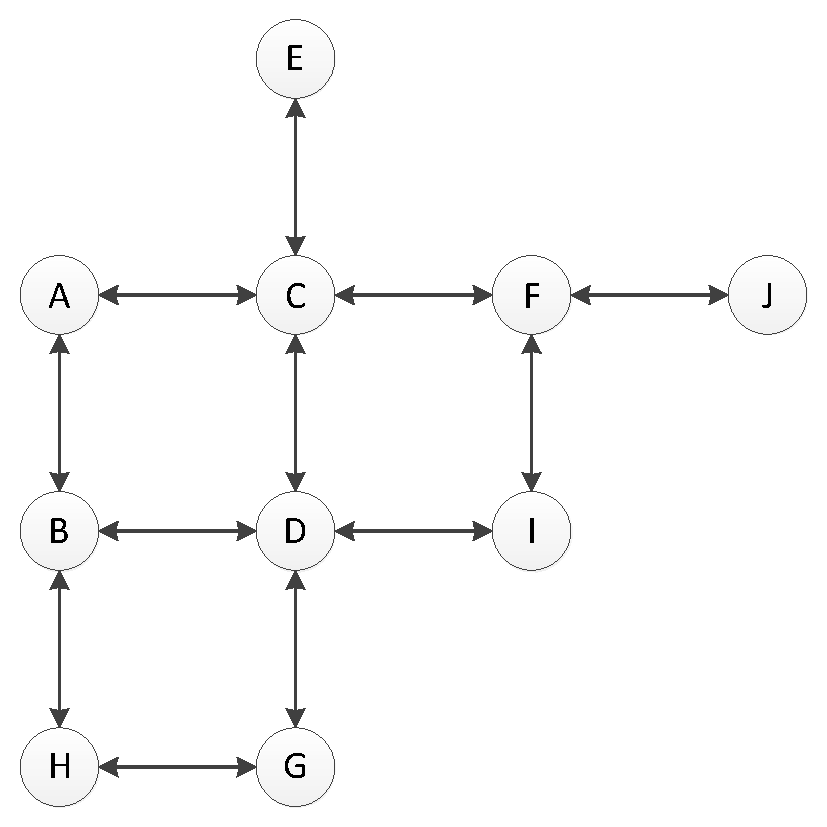
\includegraphics[width=0.45\textwidth]{Diagrams/neighbour-network}}
\subfigure[Logical Tree imposed on network when aggregating neighbours]{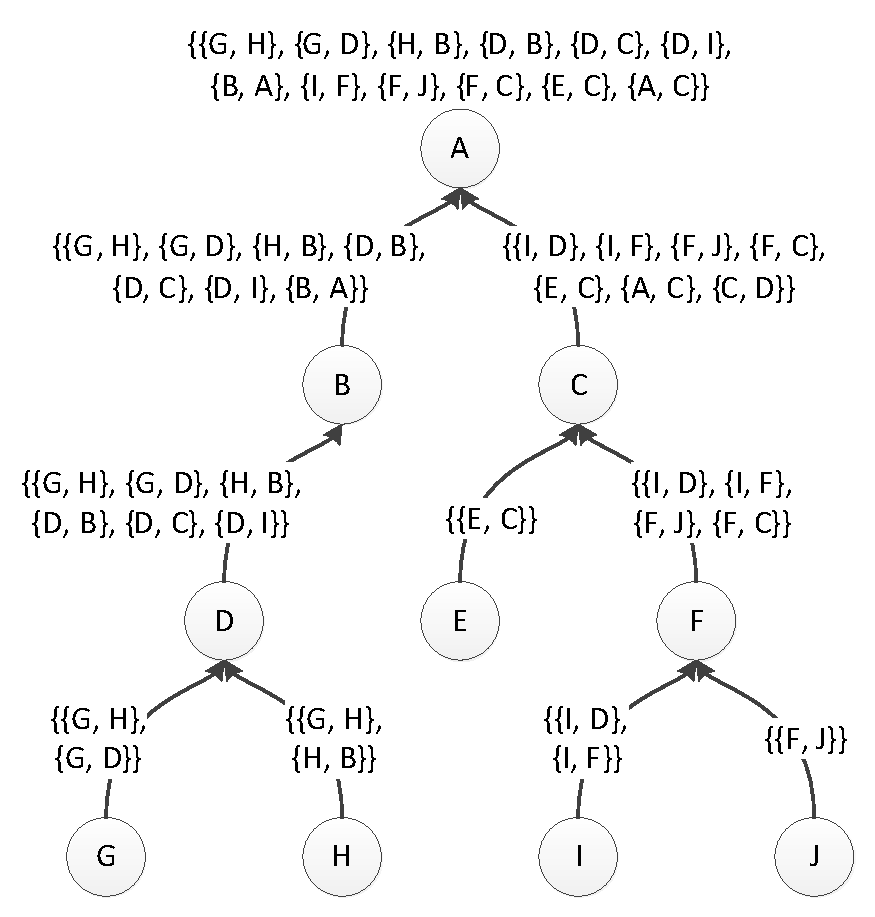
\includegraphics[width=0.45\textwidth]{Diagrams/neighbour-tree-structure}}
\end{figure}

\subsubsection{Neighbour Detect}

To aid in debugging a vital piece of information that will be required about the network is its topology. Trying to analyse network state without knowing which nodes are neighbours of other nodes, makes drawing meaningful conclusions from that data much harder. This meant that we needed a way to send neighbour information back to the sink. Thankfully part of the job is already accomplished as Contiki comes with a library to perform neighbour detection\cite{?}. We extended that library in two ways.

The first was to add more features to Contiki's neighbour detect library. As that library was very simple and supported only saying that a neighbour had been detected (with the option of providing a integer value as well). As we were aiming for this code to support changes in the network, such as nodes leaving or joining neighbourhoods, we added the concept of a round. Instead of just knowing about neighbours at that instant in time, it allowed the library to maintain some kind of history about what nodes were neighbours of other nodes in the past. Whenever new nodes are detected they are recorded, however, if a node has not been detected for a certain number of rounds then that node is removed from the record.

For this to be useful we needed a way to get this data back to the sink node. There are many ways to do this, but one of the best is aggregating along a tree because it can combine many messages into a single one and forward that aggregated message instead of lots of smaller messages \cite{1628365}. The Neighbour Aggregation part uses the Tree Aggregation library that we have developed, the function that is used to aggregate data together is $\cup$ (union), this allows data to be aggregated with other data and allows that data to be updated. The nodes own data is set to be $\res{node-data}$, where $\var{j}$ is the current node's address and $\res{round-data}$ is the set of node addresses provided by the $\res{neighbour-detect.callback}$ callback in \autoref{algo:neighbour-detect}.

\begin{equation}
\res{node-data} = \{\{\var{other}, \var{j}\} | \var{other} \in \res{round-data} \}
\end{equation}

\begin{figure}[H]
  \centering
  \begin{boxedminipage}{\linewidth}
    % 
    \null Process $j$ - \res{neighbour-detect}\\
    %
    \null \textbf{variables}\\
    %
    \null\qq \var{period}: timer init $P_{round}$;\\~\\
    %
    \null\qq \% The history of node\\
    \null\qq \var{previous}: map of address to int init $\emptyset$;\\~\\
    %
    \null\qq \% The current round\\
    \null\qq \var{count}: int init 0;\\~\\
    %
    \null \textbf{constants}\\
    %
    \null\qq \% Round Period\\
    \null\qq \var{$P_{round}$}: time;\\~\\
    %
    \null\qq \% The missed round threshold\\
    \null\qq \var{missed}: int;\\~\\
    %
    \null \textbf{actions}\\
    %
    %
    \null\qq \% Check for changes\\
    \null\qq \emph{round}::~\res{timeout}(\var{period}) $\rightarrow$\\
    \null\qq\qq $\var{previous} \assign \{ (addr, round) \in \var{previous} | count - round \geq missed \}$;\\
    \null\qq\qq \% Tell library caller that a round is finished\\
    \null\qq\qq \res{neighbour-detect.callback}(\res{values}(previous), \var{count});\\
    \null\qq\qq $\var{count} \assign \var{count} + 1$; \\
    \null\qq\qq \res{set}($\mathit{period}$, $P_{round}$); \\~\\
    %
    %
    \null\qq \% Receiving Neighbour Discovery message\\
    \null\qq \emph{neighbour}::~\res{neighbour-discovery.recv}$\langle source, round\rangle \rightarrow$\\
    \null\qq\qq \% Update the round we last saw this node\\
    \null\qq\qq \res{if} ($source \in \res{keys}(\var{previous})$) \res{then} \\
    \null\qq\qq\qq \res{if} ($round > \var{previous}[\var{source}]$) \res{then} \\
    \null\qq\qq\qq\qq $\var{previous}[\var{source}] \assign \var{round}$; \\
    \null\qq\qq\qq \res{fi}; \\
    \null\qq\qq \res{else} \\
    \null\qq\qq\qq $\var{previous}[\var{source}] \assign \var{round}$; \\
    \null\qq\qq \res{fi}; \\
    %
    %
  \end{boxedminipage}
  \caption{Neighbour Detect Algorithm}
  \label{algo:neighbour-detect}
\end{figure}

% We can't include this because we never use or refer to these algorithms
\begin{comment}
\subsection{Clustering}

\begin{figure}[H]
  \centering
  \begin{boxedminipage}{\linewidth}
    % 
    \null Process $j$ - \res{clustering}\\
    %
    \null \textbf{variables}\\
    %
    \null\qq \% Boolean set to true when a node is elected to be a clusterhead\\
    \null\qq \var{is\_CH}: bool init $False$;\\~\\
    %
    \null\qq \% Bool set to true on receipt of first setup message\\
    \null\qq \var{seen\_setup}: bool init $False$;\\~\\
    %
    \null\qq \% Hop distance to best clusterhead\\
    \null\qq \var{best\_hop}: int;\\~\\
    %
    \null\qq \% Address of best clusterhead\\
    \null\qq \var{our\_CH}: address;\\~\\
    %
    \null\qq \% Newest setup message received\\
    \null\qq \var{msg}: struct;\\~\\
    %
    \null \textbf{constants}\\
    %
    \null\qq \% Detection Time, how long to wait for a better parent after hearing a setup message\\
    \null\qq \var{$T_{detect}$}: time;\\~\\
    %
    \null \textbf{actions}\\
    %
    %
    \null\qq \% Receive new setup message\\
    \null\qq \emph{receive-setup}::~\res{recv}$\langle source, CH, hops\rangle \rightarrow$\\
    \null\qq\qq \% Begin detection timer if this is the first setup message seen\\
    \null\qq\qq \res{if} (!$seen\_setup$) \res{then} \\
    \null\qq\qq\qq $\var{seen\_setup} \assign True$;\\
    \null\qq\qq\qq \% Node elects itself as a CH if the sink is one hop away\\
    \null\qq\qq\qq $\var{is\_CH} \assign msg.hops == 1$;\\
    \null\qq\qq\qq \res{if} ($is\_CH$) \res{then} \\
    \null\qq\qq\qq\qq \res{CH\_detect\_finished}(); \\
    \null\qq\qq\qq \res{else}\\
    \null\qq\qq\qq\qq \res{ctimer\_set}($T_{detect}$,CH\_detect\_finished); \\
    \null\qq\qq \res{fi}; \\
    \null\qq\qq \res{if} ($msg.hops < tmp\_hop\_count$ \&\& !$is\_CH$) \res{then} \\
    \null\qq\qq\qq $\var{tmp\_CH} \assign \var{msg.source}$;\\
    \null\qq\qq\qq $\var{tmp\_best\_hop} \assign \var{msg.hops}$;\\~\\
    %
    %
    \null\qq \% End detection period, finalise values\\
    \null\qq \emph{CH\_detect\_finished}::~\res{timeout}(\var{T\_detect}) $\rightarrow$\\
    \null\qq\qq $\var{our\_CH} \assign \var{tmp\_CH}$;\\
    \null\qq\qq $\var{best\_hop} \assign \var{tmp\_best\_hop}$;\\
    \null\qq\qq \% Forward the setup message\\
    \null\qq\qq $\var{newmsg.source} \assign \var{\j}$;\\
    \null\qq\qq $\var{newmsg.CH} \assign \var{is\_CH ? j : our\_CH}$;\\
    \null\qq\qq $\var{newmsg.hops} \assign \var{best\_hop}+1$;\\
    \null\qq\qq \res{stbroadcast\_send\_stubborn}($\var{newmsg}$);\\
    \null\qq\qq \% Inform calling application that setup is complete\\
    \null\qq\qq \res{setup\_complete}();\\~\\
    %
    %
    \null\qq \% Send message placed in buffer by calling application\\
	\null\qq \emph{cluster\_send}::~\res{recv}(\var{newmsg}) $\rightarrow$\\
    \null\qq\qq \res{if} ($is\_CH$) \res{then} \\
    \null\qq\qq\qq \res{runicast\_send}($\var{sink}, \var{newmsg}$);\\
    \null\qq\qq \res{else}\\    
    \null\qq\qq\qq \res{mesh\_send}($\var{our\_CH}, \var{newmsg}$);\\
    \null\qq\qq \res{fi}; \\
  \end{boxedminipage}
  \caption{Clustering Algorithm}
\end{figure}

In a wireless network, message collisions are a significant factor in terms of decreasing performance; collisions are more likely in environments featuring a high density of messages. The intuitive solution to this is to reduce the number of messages sent, with minimal compromise in the richness of the data communicated. To this end, we implemented a clustering algorithm. The principle of operation of a clustering algorithm is to establish a set of clusterheads on network initialisation. Each of the other nodes in the network allocates itself exactly one clusterhead, through which all traffic to the sink is routed.

In our implementation, the network initialisation phase occurs when an application running on the nodes begins; this application calls the cluster setup routine. The clusterheads are selected to be the set of nodes in the one-hop neighbourhood of the sink. These nodes broadcast their status as a clusterhead to the rest of the network, and the nodes decide with which clusterhead to align themselves based on shortest distance (in hops). Throughout the remainder of the network's operation, each node passes its messages to the sink through its chosen clusterhead. At this point control is passed back to the application, which can then call the relevant functions to send a message from a node to the sink through that node's clusterhead. As the nature of the setup guarantees that clusterheads will be within one hop of the sink, the messages they pass on from their respective nodes are sent using Contiki's runicast message type. There are no such guarantees for the other nodes, so Contiki's mesh routing is used to allow for arbitrary distance between a node and its clusterhead. This approach to clustering works well when used in small networks, as it achieves its main goal of reducing the number of messages being passed (specifically, the medium will be a lot less congested in the one-hop neighbourhood of the sink). However, this algorithm clearly does not scale well with either geographical distance or number of nodes. In the former case, the majority of nodes will be out of direct transmission range of their clusterhead and will thus have to route messages through several other intermediary nodes; thus increasing the number of messages in the network. Similarly, with large networks a large number of nodes will all need to send messages to clusterheads which form an increasingly small proportion of the network; this is liable to cause bottlenecks and collisions.

\subsection{Hierarchical Clustering}


\begin{figure}[H]
  \centering
  \begin{boxedminipage}{\linewidth}
    % 
    \null Process $j$ - \res{hierarchical-clustering}\\
    %
    \null \textbf{variables}\\
    %
    \null\qq \% Boolean set to true when a node is elected to be a clusterhead\\
    \null\qq \var{is\_CH}: bool init $False$;\\~\\
    %
    \null\qq \% Bool set to true on receipt of first setup message\\
    \null\qq \var{seen\_setup}: bool init $False$;\\~\\
    %
    \null\qq \% Hop distance to best clusterhead\\
    \null\qq \var{best\_hop}: int;\\~\\
    %
    \null\qq \% Address of best clusterhead\\
    \null\qq \var{our\_CH}: address;\\~\\
    %
    \null\qq \% The number of clusterheads above the node in the hierarchy\\
    \null\qq \var{our\_level}: int;\\~\\
    %
    \null\qq \% Newest setup message received\\
    \null\qq \var{msg}: struct;\\~\\
    %
    \null \textbf{constants}\\
    %
    \null\qq \% Detection Time, how long to wait for a better parent after hearing a setup message\\
    \null\qq \var{$T_{detect}$}: time;\\~\\
    %
    \null\qq \% Cluster depth, the number of hops in a cluster before a new level is created\\
    \null\qq \var{$depth$}: time;\\~\\
    %
    \null \textbf{actions}\\
    %
    %
    \null\qq \% Receive new setup message\\
    \null\qq \emph{receive-setup}::~\res{recv}$\langle source, CH, CH\_level, hops\rangle \rightarrow$\\
    \null\qq\qq \% Begin detection timer if this is the first setup message seen\\
    \null\qq\qq \res{if} (!$seen\_setup$) \res{then} \\
    \null\qq\qq\qq $\var{tmp\_best\_level} \assign \var{msg.CH\_level}$;\\
    \null\qq\qq\qq $\var{tmp\_CH} \assign \var{msg.CH}$;\\
    \null\qq\qq\qq $\var{tmp\_best\_hop} \assign \var{msg.hops}$;\\
    \null\qq\qq\qq \res{ctimer\_set}($T_{detect}$,CH\_detect\_finished); \\
    \null\qq\qq \res{fi}; \\
    \null\qq\qq \res{if} ($msg.hops < tmp\_hop\_count$ \&\& $msg.CH\_level \leq tmp\_best\_level$) \res{then} \\
    \null\qq\qq\qq $\var{tmp\_CH} \assign \var{msg.CH}$;\\
    \null\qq\qq\qq $\var{tmp\_best\_hop} \assign \var{msg.hops}$;\\
    \null\qq\qq\qq $\var{tmp\_best\_level} \assign \var{msg.CH\_level}$;\\
    %
    %
    \null\qq \% End detection period, finalise values\\
    \null\qq \emph{CH\_detect\_finished}::~\res{timeout}(\var{T\_detect}) $\rightarrow$\\
    \null\qq\qq $\var{our\_CH} \assign \var{tmp\_CH}$;\\
    \null\qq\qq $\var{best\_hop} \assign \var{tmp\_best\_hop}$;\\
    \null\qq\qq $\var{is\_CH} \assign \var{best\_hop} == \var{depth}$;\\
    \null\qq\qq $\var{our\_level} \assign \var{is\_CH}? \var{tmp\_best\_level} + 1 : \var{tmp\_best\_level}$;\\
    \null\qq\qq \% Forward setup message after a pseudorandom wait period\\
    \null\qq\qq \res{forward\_setup}();\\
    %
    %
    \null\qq \% Forward setup message through the network\\
    \null\qq \emph{forward\_setup}::~\res{timeout}(pseudorandom-delay) $\rightarrow$\\
    \null\qq\qq $\var{newmsg.source} \assign \var{\j}$;\\
    \null\qq\qq $\var{newmsg.CH} \assign \var{is\_CH ? j : our\_CH}$;\\
    \null\qq\qq $\var{newmsg.CH\_level} \assign \var{our\_level}$;\\
    \null\qq\qq $\var{newmsg.hops} \assign \var{is\_CH} ? 0 : \var{best\_hop}+1$;\\
    \null\qq\qq \res{stbroadcast\_send\_stubborn}($\var{newmsg}$);\\
    \null\qq\qq \% Inform calling application that setup is complete\\
    \null\qq\qq \res{setup\_complete}();\\
    %
    %
    \null\qq \% Send message placed in buffer by calling application\\
	\null\qq \emph{cluster\_send}::~\res{recv}(\var{newmsg}) $\rightarrow$\\
    \null\qq\qq \res{if} ($best\_hop == 1$) \res{then} \\
    \null\qq\qq\qq \res{runicast\_send}($\var{our\_CH}, \var{newmsg}$);
    \null\qq\qq \res{else}\\    
    \null\qq\qq\qq \res{mesh\_send}($\var{our\_CH}, \var{newmsg}$);
    \null\qq\qq \res{fi}; \\
  \end{boxedminipage}
  \caption{Hierarchical Clustering Algorithm}
\end{figure}

To counter the given disadvantages of our basic clustering implementation, we developed an additional algorithm which employs the concept of hierarchical clustering. That is, a cluster featuring multiple layers of clusters, each with  clusterhead that has a clusterhead of its own in the next layer. The setup phase of this algorithm also chooses the one-hop neighbourhood of the sink as clusterheads. However, when these clusterheads' setup messages are broadcast through the network, if a node detects that its nearest clusterhead is at least $d$ hops away –- where $d$ is defined as a constant in \verb|contiki.c| –- then that node elects itself as a clusterhead of a new layer, and generates its own setup message to be broadcast. We initially designed two versions of hierarchical clustering; one for arbitrary values of $d$, and one for $d=1$ (where every non-leaf node becomes a clusterhead). However, once the former version was finished we decided to consolidate both versions into one and simply treat $d=1$ as a specific case. To avoid the potential problem of mesh routing creating more messages than the hierarchical clustering saves, in cases of any node being within direct range of its clusterhead, it transmits using runicast. In all other cases, the node uses mesh as before. The hierarchical approach removes the major limitations of our initial clustering implementation, however it still suffers from selecting permanent clusterheads (whereas methods such as LEACH\cite{LEACH} randomise the clusterheads periodically) and thus causing increased power usage for these nodes. Unfortunately, given that we developed our clustering implementation as a library to be used by some arbitrary application running on the nodes, the process of reassigning clusterheads (in any manner of synchronisation) proved infeasible.
\end{comment}
% End of what we can't include

\subsection{TDMA}

To have a representative algorithm of what may be tested, TDMA (Time Division Multiple Access) was chosen to be implemented and have predicates written for it. The algorithm that was initially implemented was described by \citeauthor{DCATechReport} in \cite[p.~4]{DCATechReport} and is outlined below:

\begin{enumerate}
\item Initially assign every node the smallest numbered channel
\item Every round every node broadcasts a message containing their ID and their currently assigned channel
\item When a message is received the neighbour set is updated and the node that received the message assigns its channel to be the lowest channel not assigned to any neighbour. Two neighbours are not allowed to change their channel in the same round, so a tie breaker is done and the node with the lower ID is allowed to change their channel
\item After choosing a channel the node broadcasts its ID and chosen channel
\item The procedure is repeated until every node cannot choose a smaller channel than its current channel
\end{enumerate}

Interestingly enough when this was first implemented the algorithm only made sure that a node did not have the same channel as any of its one hop neighbours. It did not ensure that the one hop neighbours of any node would have unique channels (as would be required by TDMA to ensure no collisions). This is the kind of bug that running predicates would have assisted identifying.

To make sure that the channel allocation was suitable for TDMA, instead of nodes just sending their own channel assignment to its neighbours. It also included the assignment of the one hop neighbours it knows about in that message. This then allowed nodes to receive information on their two hop neighbourhoods, which they then based their decision on what channel to allocate to themselves from.

\subsection{Testing}

When testing our implementations there were a number of difficulties due to the differences in what was being tested, how that library needed to tested and under what circumstances. For the containers library we wrote a number of tests that simply created the relevant container and then performed an action on it. The test succeeded if the state of the container was as expected after the execution of the test. These tests were run under various conditions, including under valgrind to ensure that there were no memory leaks in these critical pieces of code.

The remaining libraries were difficult to test because they were communication libraries, so we developed applications that used them and made sure that in our tests these application performed as expected. To test Tree Aggregation without large packet support we developed a simple temperature and humidity averaging application. To test Tree Aggregation with large packet support (from our multi-packet library) we developed an application to aggregate neighbours back to the base station. This is the same application that we integrated as the neighbour detection library because it became vital for performing predicate evaluation at the base station.

N-Hop Flood, N-Hop Request and Event Update were all tested as part of the behaviour of the relevant predicate evaluation library they were used in (PELE, PELP and PELE respectively). The libraries were developed to ensure that we had correctly encapsulated the required functionality which meant that if we discovered an issue in one component we knew where we would need to look for the error.

When testing for memory leaks we couldn't use the same approach as used to test the container libraries. This is because sensor network application never truly terminate, meaning there is no good point to check that all the memory allocated has been freed. What we instead did was run the applications we had developed in the simulators for a long period of time until the application crashed. We then used the stack trace to work out where the error was and fix that component. For memory leaks we also had to manually inspect all the allocation and freeing routines to ensure that the memory that was allocated is freed.

\subsection{Visualisation Tool}

In order to interface with WSNs, we require software which can run on the base--station attached to sink node, and communicate back and forth with said node. We have developed a Java GUI tool for this purpose. It's main functions include creating predicates to be monitored, deploying these predicates to the WSN, and aggregating the results across multiple rounds of evaluation in an easy to use interface.

The tool has two main views, predicate view and network view. As shown in (TODO insert figures). Predicate view provides a list of predicates along with their status (satisfied, unsatisifed, unmonitored etc.), source code (written in our predicate scripting language), and more detailed evaluation results when available.

The network view on the other hand displays a visualisation of the WSN as a graph --- with vertices representing nodes and edges representing neighbour relationships.

The user can scroll freely back and forth between previous rounds and view the data contained in each view for any of them.

\subsection{Summary}

Either we were unable to find implementations of what we needed or it simply hadn't been implemented, this unfortunately added a lot of development time to this project. We were very shocked that libraries such as tree aggregation and hop-limited flooding seemed unavailable in Contiki as we thought that these would be fundamental libraries for wireless sensor network development. Drawing parallels from recent developments in C++ standardisation, the committees involved are actively seeking new libraries to include in the next standard due to the benefit it brings the language \cite{c++call-for-proposals}. We believe that if Contiki supported a number of additional containers other than a linked list and circular buffer as well as other higher-level networking libraries in RIME, then Contiki could be much more useful. We will be looking to see if we can contribute back anything we have developed.

